\noindent
\includegraphics[height=1.25cm]{images/pictograms/benchmark}
\includegraphics[height=1.25cm]{images/pictograms/FEM}

%%%%%%%%%%%%%%%%%%%%%%%%%%%%%%%%%%%%%%%%%%%%%%%%%%%%%%%%%%%%%%%%%%%%%%%%%%%%%%%%%%%%%%%%%%%%%%%%%%%

\begin{flushright} {\tiny {\color{gray} python\_codes/fieldstone\_176/text.tex}} \end{flushright}

%\lstinputlisting[language=bash,basicstyle=\small]{python_codes/template_keywords.key}

\par\noindent\rule{\textwidth}{0.4pt}

\begin{center}
\inpython
{\small Code: \url{https://github.com/cedrict/fieldstone/tree/master/python_codes/fieldstone_176}}
\end{center}

\par\noindent\rule{\textwidth}{0.4pt}

Last revision: July. 21st, 2026.

\par\noindent\rule{\textwidth}{0.4pt}

{\sl This stone was developed based on an idea by Mohit Lohani}. \index{contributors}{M. Lohani}

\par\noindent\rule{\textwidth}{0.4pt}

%%%%%%%%%%%%%%%%%%%%%%%%%%%%%%%%%%%%%%%%%%%%%%%%%%%%%%%%%%%%%%%%%%%%%%%%%%%%%%%%%%%%%%%%%%%%%%%%%%%

This \stone is based on \stone~1. It has been modified slightly to make it more compact
(explicit for loops have been removed for a great deal) without
changing any functionality at all (note however that no graphical output is produced).

What I will test here is the assembly process algorithm. Indeed \stone~150 showed us that 
it is a part of a FEM code that is time demanding and difficult to optimize. 
I am here testing an approach that one of my students used in class.

I then choose for the simplest and easiest case of the penalty formulation that yields a FEM system that 
is not a saddle point system. No vtu file is produced since it is not needed here.

%-------------------------------------------
\subsection*{Implementation - The `old' way}

The FE matrix is defined as a Row-based LIst of Lists sparse 
matrix\footnote{\url{https://docs.scipy.org/doc/scipy/reference/generated/scipy.sparse.lil_matrix.html}}:
\begin{lstlisting}
a_mat = lil_matrix((Nfem,Nfem),dtype=np.float64)
\end{lstlisting}
Inside the loop over elements the elemental matrix \lstinline{a_el} is built
and the assembly is as follows:

\begin{lstlisting}
for k1 in range(0,m):
    for i1 in range(0,ndof):
        ikk=ndof*k1          +i1
        m1 =ndof*icon[k1,iel]+i1
        for k2 in range(0,m):
            for i2 in range(0,ndof):
                jkk=ndof*k2          +i2
                m2 =ndof*icon[k2,iel]+i2
                a_mat[m1,m2]+=a_el[ikk,jkk]
            #end for
        #end for
        rhs[m1]+=b_el[ikk]
    #end for
#end for
\end{lstlisting}
The quadruple for loop is not conducive to a fast python code.

Finally the matrix is converted to CSR format:
\begin{lstlisting}
A=sps.csr_matrix(a_mat)
\end{lstlisting}
before being passed to the solver alongside the rhs vector:
\begin{lstlisting}
sol=sps.linalg.spsolve(A,rhs)
\end{lstlisting}

%-------------------------------------------
\subsection*{Implementation - The `new' way}

In this case the matrix is defined as follows, along side two 
required arrays that will store the entries locations:
\begin{lstlisting}
row = [] 
col = []
a_mat = []
\end{lstlisting}
Note that here the matrix is a one-dimensional array
while it was a two-dimensional one in the previous case.
Then, the assembly is as follows (note the required \lstinline{dofs}
array that contains the list of all dofs for the element under consideration:
\begin{lstlisting}
for iel in range(0,nel):
    ...
    for k in range(0,m):
        dofs[k*ndof+0]=icon[k,iel]*ndof+0
        dofs[k*ndof+1]=icon[k,iel]*ndof+1
    ...
    for i_local,idof in enumerate(dofs):
        for j_local,jdof in enumerate(dofs):
            row.append(idof)
            col.append(jdof)
            a_mat.append(a_el[i_local,j_local])
        #end for
        rhs[idof]+=b_el[i_local]
    #end for
\end{lstlisting}
We have used here the python \lstinline{enumerate} functionality. In fact
\begin{lstlisting}
for i_local,idof in enumerate(dofs):
\end{lstlisting}
elegantly replaces
\begin{lstlisting}
for i_local in (0,m):
    idof=dofs[i_local]
\end{lstlisting}
Finally the CSR converstion goes as follows:
\begin{lstlisting}
A=sps.csr_matrix((a_mat,(row,col)),shape=(Nfem,Nfem))
\end{lstlisting}


%-------------------------------------------
\subsection*{Results/timings}

The bash {\tt script\_errors} runs the code over a range of resolutions 
and for each resolution runs it 4 times so as to obtain better average 
timings. Various parts of the code are timed and we compare values between 
the `old' and the `new' approach. Results have been obtained on my 
laptop (Lenovo ThinkPad T470p, with Intel Core i7-7820HQ CPU at 2.90GHzx8),
and on Shrek (Intel Xeon E5-2660 v3x40).

Let us start with the assembly:
\begin{center}
\includegraphics[width=8cm]{python_codes/fieldstone_176/results/assembly.pdf}
\includegraphics[width=8cm]{python_codes/fieldstone_176/results/convert2csr.pdf}\\
{\captionfont Left: time required to carry out the assembly; Right: time
required to carry out the CSR conversion.}
\end{center}
We find that the new method yields an assembly about 10x faster 
but the CSR conversion is then more than 10x slower. 

In context, one can now look at the total time needed to build the matrix,
as well as the solve time:
\begin{center}
\includegraphics[width=8.5cm]{python_codes/fieldstone_176/results/build.pdf}
\includegraphics[width=8.5cm]{python_codes/fieldstone_176/results/solve.pdf}\\
{\captionfont Left: time to build; Right: time to solve.}
\end{center}
The conclusion is then clear: the new method yields a matrix build that 
is about 2x faster than the old one.
Also, comparing matrix building times to solve times, we get a feel for how 
improving the assembly process ultimately makes our code faster!
\begin{center}
\includegraphics[width=10cm]{python_codes/fieldstone_176/results/build_solve.pdf}
\end{center}

\newpage
We can also monitor the time necessary to split the solution vector
and the time required to compute the pressure and strain rate components:
\begin{center}
\includegraphics[width=8cm]{python_codes/fieldstone_176/results/split.pdf}
\includegraphics[width=8cm]{python_codes/fieldstone_176/results/compute_press_sr.pdf}\\
{\captionfont We of course retrieve the same time for both implementations since
these algorithms are not linked to the assembly process.}
\end{center}
We find that the split time is negligble. 


Finally we make sure that the discretization errors converge at the expected rate
in both implementations:
\begin{center}
\includegraphics[width=8cm]{python_codes/fieldstone_176/results/errv.pdf}
\includegraphics[width=8cm]{python_codes/fieldstone_176/results/errp.pdf}\\
{\captionfont We of course retrieve the same errors for both implementations.}
\end{center}
